\documentclass{article}

\usepackage[main=english,vietnamese]{babel}
\usepackage[T1]{fontenc}
\usepackage[utf8]{inputenc}
\usepackage[sexy]{evan}
\usepackage{matchsticks}
\usepackage{wrapfig}
\usepackage{listings}

\title{Basic Math Operations}
\begin{otherlanguage}{vietnamese}
\author{Ngô Văn Minh - (Archimedes Academy)}
\end{otherlanguage}
\date{\today}

\begin{document}

\maketitle

In the last article of this series, you have learned what is counting and how to use it.
In this article, we will dive into some other basic mathematical concepts: elementary arithmetic oerations.
At the end, you will learn how to use these operations as easy as you have learned about counting.

\bigbreak

There are \textbf{four elementary arithmetic operations}:
addition (written by using the plus sign $+$), subtraction ($-$), multiplication ($\times$ or $\cdot$ or $*$),
and division ($\div$ or $/$).
\begin{itemize}[topsep=0pt, partopsep=0pt, itemsep=0pt]
    \ii \textbf{Addition}: Addition is an arithmetic operation that combines objects from two different collections.
    Addition is denoted by the plus sign $+.$


    \textit{For example, addition is a combination of three apples and two apples, making a total of five apples.
This observation is equivalent to the mathematical expression $3 + 2 = 5.$}

    \ii \textbf{Subtraction}: Subtraction is an arithmetic operation that represents the operation of removing objects from a collection.
    Subtraction is signified by the minus sign $-.$
    
    \textit{For example, subtraction is to take two apples away from a pile of five apples, resulting in a remaining pile with three apples.
    The difference of 5 and 2 is 3; that is, $5 - 2 = 3.$}
    
    \ii \textbf{Multiplication}: 
    The multiplication of two numbers is equivalent to adding as many copies of one of them, the multiplicand, as the quantity of the other one, the multiplier. Both numbers can be referred to as factors.
    \[ 
        a \times b = \underbrace{b+b +\ldots +b}_{a \text{\ times\ }}.
    \]
    
    \textit{For example, 4 multiplied by 3 is written as $3\times 4=4+4+4=12.$}

    \ii \textbf{Division}: division is a process of calculating the number of times one number is contained within another.
    This number of times need not be an integer.
    
    \textit{For example, if $20$ apples are divided evenly between $4$ people, everyone receives $5$ apples.}    
\end{itemize}

\bigbreak

Some \textbf{important properties} of the operations:
\begin{itemize}[topsep=0pt, partopsep=0pt, itemsep=0pt]
    \ii Addition and multiplication are \textit{commutative}, meaning that order does not matter:
    \[
        a + b = b + a \quad \text{\ and\ } \quad a \times b = b \times a.
    \]

    \ii Addition and multiplication are also \textit{associative},
    meaning that when one uses the operation for more than two numbers,
    the order in which the operation is performed does not matter:
    \[
        (a + b) + c = a + (b + c) \quad \text{\ and\ } \quad (a \times b) \times c = a \times (b \times c).
    \]

    \ii Multiplication is \textit{distributive} over addition:
    \[
        a \times (b + c) = a \times b + a \times c.
    \]
\end{itemize}

\newpage

\begin{example*}[Problem 1]
    \label{example:pi-2022-3-p1}
    Using only the digit $8$ and the addition operation,
    is it possible to obtaine a result of $1000$?
\end{example*}

\begin{remark*}
    There are two approaches to this problem.
    
    In the \textit{first approach}, one might observe that $1000$ is a multiple of $8,$
    thus it is a sum of a number of $8$.

    The \textit{second approach} looks at a block of $8$ as a number consisting of multiple digits of $8$
    and perhaps, finding a way to sum these blocks up to be $1000.$
\end{remark*}

\begin{soln}[Solution 1] \nameref{example:pi-2022-3-p1}
    \[ 
        \underbrace{8+8+8+\ldots+8}_{125 \text{\ digits of\ } 8}=1000.
    \]
\end{soln}

\begin{soln}[Solution 2] \nameref{example:pi-2022-3-p1}
    \[
        888+88+8+8+8 = 1000.
    \]
\end{soln}

\begin{example*}[Problem 2]
    \label{example:pi-2022-3-p2}
    The \Cref{fig:pi-2022-3-p2} below is made of a number of blocks. Some are hidden from sight.
    How many blocks are there?
\end{example*}

\begin{figure}[h]
    \centering
    \begin{minipage}[t]{6.5cm}
        \centering
        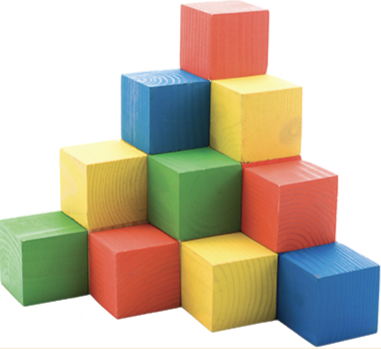
\includegraphics[width=5cm]{./png/pi-2022-3-p2.png}
        \caption{\nameref{example:pi-2022-3-p2}}
        \label{fig:pi-2022-3-p2}
    \end{minipage}
\end{figure}

\begin{soln} \nameref{example:pi-2022-3-p2}
    There are $4$ vertical layers in the figure.
    The $4^{\text{th}}$ layer (the top one) has $1$ block,
    the $3^{\text{rd}}$ layer has $1+2$ blocks,
    the $2^{\text{nd}}$ layer has $1+2+3$ blocks,
    and the $1^{\text{st}}$ layer has $1+2+3+4$ blocks.
    
    Thus, in total there are: \framebox{$1+(1+2)+(1+2+3)+(1+2+3+4)=1+3+6+10=20$} blocks.
\end{soln}

\newpage

\begin{example*}[Problem 3]
    \label{example:pi-2022-3-p3}
    Trang goes to elementary school.
    In January $2021,$ her age is equal to the sum of digits of her birth year.
    What year was she born?
\end{example*}

\begin{soln} \nameref{example:pi-2022-3-p3}
    Let the year when Trang was born be $\overline{20ab}.$
    Since Trang's age is equal to the sum of the digits of her birth year:
    \[
        2021 - \overline{20ab} = 2 + 0 + a + b
        \Rightarrow 21 - 10a - b = 2+a+b
        \Rightarrow 11a + 2b = 19
        \Rightarrow a = 1 \text{\ and\ } b = 4
    \]
    Thus, Trang was born in \framebox{$2014$}.
\end{soln}

\begin{example*}[Problem 4]
    \label{example:pi-2022-3-p4}
    Given the sequence:
    \[ 
        C+7,\  F+4,\  P-6,\  S-9,\  \_\_\_\_
    \]
    Choose the appropriate option to fill in the blank $\_\_\_\_.$
    \[
        (A) \quad B+6 \qquad
        (B) \quad I+1 \qquad
        (C) \quad K-2 \qquad
        (D) \quad R-7
    \]
\end{example*}

\begin{soln} \nameref{example:pi-2022-3-p4}
    The sequence contains a number of sums and differences of numbers and letters.
    Let consider the relation of a letter its position in the alphabet.
    Note that $C$'s position corresponds to the third, or $3$.
    $F$'s to $6$, $P$'s to $16,$ and $S$'s to $19,$ see \Cref{fig:pi-2022-3-p4}.
    
    \begin{figure}[h]
        \centering
        \begin{minipage}[t]{6.5cm}
            \begin{tabular}{cccccc}
                $A_1$ & $B_2$ & $C_3$ & $D_4$ & $E_5$ & $F_6$ \\
                $G_7$ & $H_8$ & $I_9$ & $J_{10}$ & $K_{11}$ & $L_{12}$ \\
                $M_{13}$ & $N_{14}$ & $P_{15}$ & $Q_{16}$ & $R_{17}$ & $S_{18}$ \\
                $T_{19}$ & $U_{20}$ & $V_{21}$ & $W_{22}$ & $X_{23}$ & $Y_{24}$ \\
                $Z_{25}$ &  &  &  &  & 
            \end{tabular}
            \caption{Letters' positions in the alphabet}
            \label{fig:pi-2022-3-p4}
        \end{minipage}
    \end{figure}
    
    Thus, the expressions $C+7,\ F+4,\ P-6,$ and $S-9$ all correspond to the value of $10.$
    Now, the expressions $B+6,\ K-2,\ R-7$ all correspond to the value of $9,$
    except $I+1$, which corresponds the value of $10.$
    
    Therefore, the proper value for the answer is \framebox{$B$} for $I+1.$ 
\end{soln}

\begin{example*}[Problem 5]
    \label{example:pi-2022-3-p5}
    Find the value of the operation $2022 \div 1011 \times (1+1).$
\end{example*}

\begin{soln} \nameref{example:pi-2022-3-p5}
    \[
        2022 \div 1011 \times (1+1) = 2022 \div 1011 \times 2 = 2 \times 2 = 4.
    \]
\end{soln}

\newpage

\begin{example*}[Problem 6]
    \label{example:pi-2022-3-p6}
    The \Cref{fig:pi-2022-3-p6} shows $3$ triangles made from $6$ matchsticks.
    Can you move exactly $2$ matchsticks so that there will be no triangle?
\end{example*}

\begin{figure}[h]
    \centering
    \begin{tikzpicture}
        \match{0:0}{0:3}; \match{0:0}{60:3}; \match{0:3}{120:3};
        \match{18:3}{0:3}; \match{18:3}{60:3}; \match{11:6}{120:3};
        \match{0:6}{0:3}; \match{0:6}{60:3}; \match{0:9}{120:3};
    \end{tikzpicture}
    \caption{\nameref{example:pi-2022-3-p6}}
    \label{fig:pi-2022-3-p6}
\end{figure}

\begin{soln} \nameref{example:pi-2022-3-p6}

    We observe that, geometrically, it is not possible to move $2$ matchsticks remove all $3$ triangles.
    On the other hand the difference of two equal numbers is always $0$.
    Thus, $2$ matchsticks are removed to form an equation of $\delta - \delta = 0$
 
    \begin{figure}[h]
        \centering
        \begin{tikzpicture}
            \match{0:0}{0:3}; \match{0:0}{60:3}; \match{0:3}{120:3};
            \match{18:3}{0:3}; 
            \match{0:6}{0:3}; \match{0:6}{60:3}; \match{0:9}{120:3};
            \match{6:9}{0:3}; \match{11:9}{0:3};
        \end{tikzpicture}
        \caption{$2$ matchsticks moved}
        \label{fig:pi-2022-3-p6-2}
    \end{figure}

\end{soln}

\begin{exercise*}[Exercise 1]
    \label{example:pi-2022-3-e1}
    Fill in the appropriate number into the $?$ circle of the \Cref{fig:pi-2022-3-e1} below.
\end{exercise*}

\begin{figure}[h]
    \centering
    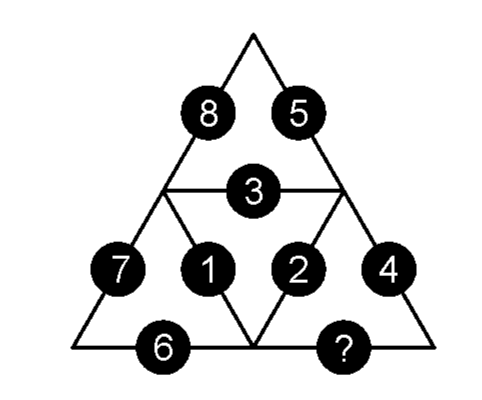
\includegraphics[width=5cm]{./png/pi-2022-3-e1.png}
    \caption{\nameref{example:pi-2022-3-e1}}
    \label{fig:pi-2022-3-e1}
\end{figure}

\begin{exercise*}[Exercise 2]
    \label{example:pi-2022-3-e2}
    Tom wrote down two positive integers, whose digits are some of the following: $1, 2, 3, 4, 5,$ and $6.$ 
    Each of the digit appeared in only one of the two numbers, and only once in that number.
    When Tom added up these numbers, he got $750.$
    What is the smallest positive integer that Tom could write?
\end{exercise*}

\begin{exercise*}[Exercise 3]
    \label{example:pi-2022-3-e3}
    A nine-digit number is created by using the digits $1, 2, 3, 4, 5, 6, 7, 8,$ and $9,$ each once.
    Every digit of the number, from the second one from the left,
    is either greater by $5$ or smaller by $4$ than the preceding one.
    How many such numbers can be created? 
\end{exercise*}

\begin{otherlanguage}{vietnamese}

\textbf{New words:}
\begin{figure}[h]
    \begin{tabular}{ll}
        {\color[HTML]{B00004} Operation}: Phép tính      & {\color[HTML]{B00004} Layer}: Tầng/lớp     \\
        {\color[HTML]{B00004} Addition}: Phép cộng      & {\color[HTML]{B00004} Correspond to}: Tương ứng với \\
        {\color[HTML]{B00004} Subtraction}: Phép trừ     & {\color[HTML]{B00004} Machstick}: Que diêm \\
        {\color[HTML]{B00004} Multiplication}: Phép nhân & {\color[HTML]{B00004} Triangle}: Tam giác  \\
        {\color[HTML]{B00004} Division}: Phép chia       & {\color[HTML]{B00004} Geometry}: Hình học  \\
        {\color[HTML]{B00004} Arithmetic}: Số học        & {\color[HTML]{B00004} Positive}: Dương     \\
        {\color[HTML]{B00004} Properties}: Các tính chất & {\color[HTML]{B00004} Integer}: Số nguyên  \\
        {\color[HTML]{B00004} Commutative}: Giao hoán    & {\color[HTML]{B00004} Digit}: Chữ số       \\
        {\color[HTML]{B00004} Associative}: Kết hợp      & {\color[HTML]{B00004} Occur}: Xuất hiện    \\
        {\color[HTML]{B00004} Analyze/Analysis}: Phân tích & {\color[HTML]{B00004} The preceding}: trước đó     
    \end{tabular}
\end{figure}

\end{otherlanguage}

\end{document}